\documentclass[letterpaper,twocolumn,10pt]{article}
\usepackage{usenix2019_v3}

% to be able to draw some self-contained figs
\usepackage{tikz}
\usepackage{amsmath}

% inlined bib file
\usepackage{filecontents}

%-------------------------------------------------------------------------------
\begin{filecontents}{\jobname.bib}
%-------------------------------------------------------------------------------
@Book{arpachiDusseau18:osbook,
  author =       {Arpaci-Dusseau, Remzi H. and Arpaci-Dusseau Andrea C.},
  title =        {Operating Systems: Three Easy Pieces},
  publisher =    {Arpaci-Dusseau Books, LLC},
  year =         2015,
  edition =      {1.00},
  note =         {\url{http://pages.cs.wisc.edu/~remzi/OSTEP/}}
}
@InProceedings{waldspurger02,
  author =       {Waldspurger, Carl A.},
  title =        {Memory resource management in {VMware ESX} server},
  booktitle =    {USENIX Symposium on Operating System Design and
                  Implementation (OSDI)},
  year =         2002,
  pages =        {181--194},
  note =         {\url{https://www.usenix.org/legacy/event/osdi02/tech/waldspurger/waldspurger.pdf}}}
\end{filecontents}

%-------------------------------------------------------------------------------
\begin{document}
%-------------------------------------------------------------------------------

%don't want date printed
\date{}

% make title bold and 14 pt font (Latex default is non-bold, 16 pt)
\title{\Large \bf Software Security Analysis of Ethereum Smart Contracts}

%for single author (just remove % characters)
\author{
{\rm Nicolas Schapeler}\\
TUM Chair of IT Security
} % end author

\maketitle

%-------------------------------------------------------------------------------
\begin{abstract}
%-------------------------------------------------------------------------------
\end{abstract}


%-------------------------------------------------------------------------------
\section{Motivation}
%-------------------------------------------------------------------------------
In recent years blockchain technology has seen more and more widespread adoption, ranging far from its initial use case of a decentralized means to exchange electronic cash, as introduced by Bitcoin. 

A key innovation in this space has been the introduction of so-called smart contracts, which were first implemented by the Ethereum protocol based on the ideas of Computer Scientist Nick Szabo. These are programs that execute automatically on the Ethereum network if certain conditions are met or if they are invoked by a blockchain participant. Through these, one can create more complex applications while still retaining the built-in trustlessness and security for which blockchain technology was initially designed. Today, smart contracts are used to automate various processes, ranging from supply chain management over energy distribution in smart grids to health care. 

The use case that provides the main motivation for this paper, however, is Finance. Here smart contracts are used to automate and enforce financial agreements between different parties, such as loan provisions, asset exchanges, and asset management amongst others. At the time of this writing, four of the top smart contracts on the Ethereum network manage around 60 Billion USD, with hundreds of other contracts overseeing multiple millions in value. Considering this in addition to the relative novelty of the field to both developers and law enforcement along with the built-in anonymity of blockchain technology applications, one can deduce why this field presents such an attractive target to malicious actors - At its current stage, performing an attack on a smart contract application often yields extremely high rewards in comparison to the risk of facing consequences. 

For these reasons, smart contracts have been the target of multiple high-profile attacks in the past years. The first large-scale attack was the DAO-Attack in 2016, where 3.6 Million Ether, worth around 50 Million USD at the time or 10 Billion USD today,  was stolen and lead to the developers of Ethereum taking the controversial action of manually reverting the attacker's exploit transactions. Other prominent attacks include the King of the Ether Throne attack in 2016 and the Parity Multisig Wallet Attack in 2017 (more details regarding the exact exploits used in these attacks are given in the Background). The reason we mention these specific attacks is that all of them exploited vulnerabilities that in hindsight appear relatively simple. The key significance, however, is that the vulnerabilities utilized are all smart contract-specific, and may therefore not be intuitively detected by a developer with lesser experience developing such applications. As previously mentioned, due to the relative novelty of smart contracts, few developers are highly experienced and are therefore prone to fall victim to already-known vulnerabilities. For this reason, we believe the software security analysis methodologies and tools disclosed in this paper are of key importance in a space where each security flaw can lead to significant financial loss: They allow for the detection of vulnerabilities the developer may not be aware of or may have overlooked. 

This Systemization of Knowledge begins by giving a brief overview of the background concepts regarding software security analysis and Ethereum smart contracts, followed by a systemization of different approaches to security fault detections, where we present and experimentally test claims regarding accuracy and performance of various existing tools. 


%-------------------------------------------------------------------------------
\section{Background}
%-------------------------------------------------------------------------------
In this section, we provide the theoretical background information related to software security analysis and Ethereum necessary for understanding the rest of this paper.

\subsection{Ethereum}
Ethereum is an open software protocol that allows for the decentralized execution of smart contracts and the exchange of value in its native cryptocurrency, Ether \footnote{Technically the unit smart contracts and accounts exchange value in is Wei, however we use Ether in the context of this paper as this makes the numbers far more manageable. ( 1 Ether = $10^{18}$ Wei) }.  These smart contracts run on the Ethereum Virtual Machine (EVM). 

\subsubsection{EVM}

The Ethereum Virtual Machine is a distributed state machine with its own set of instructions and own state at any given time. This state records all relevant information related to the Ethereum network at any given time. As one might expect, the EVM's role is to define a state transition function using its instruction set which clearly defines what next state is reached given an input state and a certain instruction to be executed. 

\subsubsection{Accounts and Smart Contracts}


In this context, a significant data structure for the Ethereum protocol is the account. This data structure has the ability to send and receive transactions, hold a balance of Ether, and interact with other smart contracts. We differentiate between two types of accounts, externally-owned accounts and smart contracts. Externally-owned accounts are generated using a public-private key-pair and can interact with the rest of the Ethereum Network using the private key's signature as proof an instruction stems from a specific account. These signed EVM instructions that accounts use to interact with one another are called transactions.  Smart Contracts, on the other hand, are deployed as pieces of software and do not come with a private-public key pair. They define a set of callable functions that other network participants can invoke. As such, a key difference between smart contracts and externally-owned accounts is that smart contracts can only perform transactions if they were first invoked by a different account. As smart contracts can be called by any account (both externally owned and other smart contracts) on the Ethereum network, it is crucial that all network participants agree what a smart contract can and cannot do. To enforce this, the code of smart contracts is strictly immutable \footnote{To be clear, only the code of smart contracts is immutable. Smart Contracts can still contain various data structures such as variables, mappings, arrays etc. which are mutable.}.

\subsubsection{Gas Fees}

As previously mentioned, the physical hardware the EVM runs on and transactions are executed on is provided by a subset of all network participants, called nodes. Since these do not want to give storage and computing power away for free, Ethereum implements a gas system, whereby each operation offered by the EVM is assigned a certain gas cost \footnote{It should be noted that taking up memory also has a certain gas cost which scales with the amount of memory taken up. This has the consequence that smart contracts are often tried to be written as concisely as possible as to avoid any unnecessary memory takeup when deploying its code onto the network and therefore spending.}. This gas is just a fee in Ether paid for the computing effort and/or storage provided by the nodes. It is important to note that the maximum an account is willing to pay for these gas fees is set by the transaction initiator, not the processing nodes. The nodes, however, have the choice of processing transactions in whatever order they please and will usually choose transactions with the highest fees and lowest effort to themselves. This means a transaction can take a significant amount of time to be processed or be rejected by the nodes altogether if the nodes believe the fees are not high enough for their expended effort. It is also to be noted, that blocks in the Ethereum Network have an upper gas limit, a limit on how much computation can be done and how much gas can be spent in one block, which can also lead to a transaction being reverted if the work performed in it costs more gas than the upper gas limit.

\subsection{Solidity}
\label{subsection:sol}
Although the smart contract representation one finds on the physical blockchain is in EVM bytecode, very few smart contracts are manually written in this form and instead employ higher-level languages. There are multiple programming languages specifically adapted for developing smart contracts, however, in the context of this paper, we set our focus on Solidity. The reason we choose this language is not only for it being the most popular [citation] but also due to it having received criticism for being designed in a way that facilitates errors that lead to security flaws in smart contract development. We introduce some of these patterns here in order to better help the reader's understanding of the types of issues the software security analysis tools detect in the Contribution section of this paper.

\begin{itemize}
  \item Inconsistent Exception handling
	
	Exceptions can be caused by various factors, such as a transaction going over its allocated gas fee limit, the EVM call stack overflowing, or the \verb|throw| command being called. However, when an exception is raised, Solidity is not consistent in how it handles these and may therefore facilitate creating vulnerabilities caused by incorrectly handling exceptions. For example, if one wants to transfer Ether from an account to another, this can be done in 3 ways: 
	\begin{enumerate}
	\item \verb|<receivingAddress>.transfer(amount)| 
	\item \verb|<receivingAddress>.send(amount)|
	\item \verb|<receivingAddress>.call().gas().value(amount)|
	\end{enumerate}
	
	These have some key differences: The \verb|transfer| method throws an exception if the transfer fails for any reason and reverts the entire transaction it was a part of. The other two, however, simply return \verb|False| on failure and do not revert the transaction. Additionally, \verb|transfer| and \verb|send| have a fixed gas fee when used, while \verb|call| can have its gas fee set by the invoker \footnote{Though we use $call$ in this context to transfer funds, the main use of this command is to invoke a smart contract's function.}. 
  \item Fallback function
  
  Smart contracts have the option of defining a so-called fallback function which is executed when receiving Ether without the sender specifying a function call\footnote{If a contract does not define such a function, it cannot receive Ether.}. Aside from being executed as a side effect to receiving Ether, this function is also executed in other situations that may seem unexpected. Given a contract $C$ with a function with the signature \verb|function f(uint) returns (byte)|, if one were to call the function \verb|function f(int) returns (byte)| (notice the incorrect signature) on $C$, the result would not be a revoked transaction, exception, or a returned \verb|False| boolean, but rather an execution of the fallback function of $C$. The same is true if one mistypes the address of $C$ and attempts to invoke the nonexistent function \verb|f| on a contract $C'$, the result is an execution of the fallback function of $C'$. 
  
  This behavior worked in conjunction with the exception handling inconsistencies to cause the King of the Ether Throne attack mentioned in the introduction. There, the essence of the attack was invoked through the usage of the previously introduced \verb|send| function in the vulnerable contract. The intention of \verb|send| in the victim contract was to simply send an amount of Ether to an address, however the programmer had forgotten about the side-effect of the invoked fallback function if the recipient is a contract. Next, the \verb|send| function's fixed gas fee was not enough to pay for the attacker's contract's fallback function fee and an exception was produced, which \verb|send| returns through the use of a boolean. The victim contract, however, had no boolean check for \verb|send|, which resulted in the victim contract finding itself in a deadlocked state.
  
    \item Reentrancy
    
    
    This vulnerability is not as much an influence of Solidity's design like the previous two examples, however we view it as one of the key attack vectors in smart contract development and therefore provide a short explanation. Assume we have two Smart Contracts:
    
  \begin{verbatim}
contract Bank{  
  mapping (address => uint) balances;

  function withdraw(uint _val) public {
    // msg.sender is the account that  
    // made the function call
    address a = msg.sender;
    // Check sufficient balance
    if(balances[a] >= _val) {
      // Send the money 
      // and check the send succeeded
      require(a.call.value(_val).gas());
      // Remove sent money from balance
      balances[msg.sender] -= _val;
      }
   }
}  

contract Attacker{
  // Fallback function,
  // executed when receiving money
  function() payable { 
    // Call Bank.withdraw again    
  }
}
  \end{verbatim}
  
As one can deduce from the provided code, the vulnerability here is that the bank first sends money to the withdrawing account before removing the sent money from the account's balance. Additionally, the bank uses the \verb|call| function to send money and does not specify a maximum gas fee. An attacker can therefore implement a more complex fallback function without the risk of their money transfer failing due to the gas fee of their fallback function being too high. The attacker leverages this by calling the withdraw function again, thereby being able to withdraw as much money as he wants from the bank contract until the bank is out of money. This sort of vulnerability is what was leveraged in the DAO Attack mentioned in the introduction. 

	\item Denial of Service using Gas Limit
	The final attack vector we seek to present is a DoS attack. Assume we have given the following contract:
	
\begin{verbatim}
contract DoS{
  address[] ads;

  function addAdr(address toAdd) { 
    ads.push(toAdd);
  }

  function f(){
    for(uint i = 0; i < ads.length; i++) { 
        // Some operation on each address
    }
  }
}
\end{verbatim}

An attacker can provoke a DoS by adding suficiently large number of addresses to the \verb|ads| array of the contract. Then, if another account seeks to execute \verb|f|, the gas cost will be so high that it surpasses the block gas limit and the execution will fail.
  
  \end{itemize}

\subsection{General Security Analysis Methodologies}

Finally, we introduce some general security analysis methodologies which adaptions to Ethereum will be presented in Section 3 of this paper. 

\subsubsection{Symbolic Execution}

Symbolic Execution functions by taking a program's source code as an input and assigning symbolic values to unknown inputs. It then executes the given program using said symbolic values and is thereby able to compute expressions for the unknown inputs along with fitting constraints belonging to each possible execution path of a program. A key limitations of symbolic execution is path explosion, where the number of possible paths to symbolically execute becomes very large very quickly for large programs, especially if these contain loops that cannot be trivially rolled out.

\subsubsection{Mutation Testing}
The goal of mutation testing is to assess the efficiency of the test suite belonging to a certain piece of software. It works by generating so-called "mutants" of the provided source code, which are clones of the original code with slight alterations (for example, a change from a $>$ to a $\geq$). Then, the given test suite is ran on these generated mutants and the amount of mutants which pass the tests is measured. Generally, a low amount of mutants passing all tests is viewed as evidence of the test suite's high quality.


%-------------------------------------------------------------------------------
\section{Security Analysis Methodologies}
%-------------------------------------------------------------------------------
In this section we present current methodologies for detecting security analysis of smart contracts, where we split the approaches into two camps; static and dynamic methodologies.


\subsection{Static Analysis Methods}
We define static analysis as analysis performed on smart contract code or bytecode performed in a non-runtime environment without direct execution of the given smart contract.


Due to the general difficulty of realizing a realistic simulation of the runtime environment of smart contracts, there is a wide array of static analysis methods. One of the reasons for this difficulty is that some Ethereum-specific security flaws stem from the outcome of operations dependent on arrival times of transactions on the blockchain, the order of which is determined by the nodes on the network and is therefore non-deterministic. Additionally, many smart contracts interact with other smart contracts and writing stubs for all of these can prove to be very time-consuming and in some cases, unfeasible.


\subsubsection{Symbolic Execution}
A technique commonly found in various automated software security analysis engines is symbolic execution. Symbolic execution provides the advantage of analyzing contract code based on available paths rather than available inputs. The amount of possible paths are often easier to generate than inputs that, depending on order, lead to differing outcomes. 

Furthermore, smart contracts generally mitigate some of the weaknesses of symbolic execution mentioned earlier: First, they are generally kept rather short, as each additional unit of memory comes with a certain gas cost when deploying onto the Ethereum network. Next, smart contracts often avoid unbounded/unconstrained loops, as these can also pose a security risk and lead to potential DoS attacks, as explained in Section ~\ref{subsection:sol}.


One of the first tools to utilize this was OYENTE. OYENTE can detect 4 types of security weaknesses: Transaction Ordering Dependences (TOD), Timestamp Dependences \footnote{This vulnerability simply refers to a contract that executes based on the block timestamp. The reason this is insecure is because the node that processes the block can vary the timestamp by up to 900 seconds from the real system time and could thereby influence the contract execution in their favor.}, Exception Mishandling, and Re-entrancy vulnerabilities. OYENTE takes two inputs, namely the EVM bytecode of the contract to be analyzed and the current global state of the Ethereum Network. Here, the latter input is used to initialize certain contract variables from the bytecode in order to ensure a more accurate base state to perform symbolic execution from. The tool thereby leverages the availability and accessibility of both these inputs, as both are stored on the Ethereum blockchain and can be obtained using most Ethereum block explorers for any given smart contract. 

\begin{figure}
\begin{center}
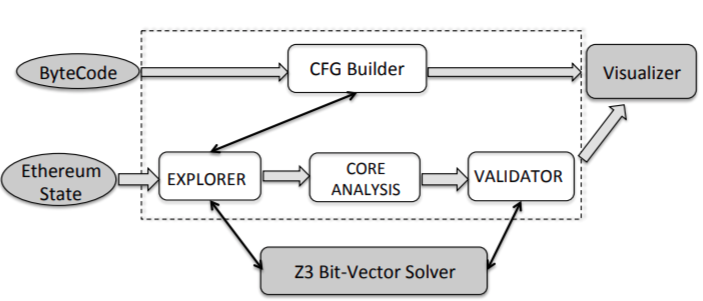
\includegraphics[scale=0.35]{oyente}
\end{center}
\caption{\label{fig:oyente} The OYENTE Tool's Structure}
\end{figure}


OYENTE works in 4 steps, depicted in Figure~\ref{fig:oyente}: First, it generates a control flow graph of the smart contract at hand which it then performs symbolic execution on. The output of this operation is then scanned for previously defined security vulnerability patterns. The product of the previous step is then filtered for false positives and finally returned to the user. OYENTE is specifically highlighted in this paper, as it was one of the first checkers in the space and designed with extendability in mind, serving as the base for multiple others [Ethir, The ones in that paper ]

\subsubsection{Visualization Tools}
The first construction of OYENTE, the Control Flow Diagram, can not only be found in most checkers employing symbolic execution but also in various other, often more lightweight, tools. The Ethereum ecosystem is compatible with various custom pieces of software used to visualize control flow, documentation, and smart contract structure amongst other things. Though these tools are not as sophisticated as symbolic analysis, they are more accessible to beginners and useful for preventing large errors along with providing simplified access to documentation. 

\subsubsection{Generic Property Verification}
A key flaw of OYENTE is its limitation of only detecting security flaws and verifying properties that are specifically hard-coded into it. However, as time passes and the Ethereum ecosystem grows, new security flaws are discovered which one wants to check for as well. The developers of OYENTE heeded this fact when they originally designed it by allowing for simple extendability, however, this still requires one to manually program an extension for OYENTE if one desires to verify a specific property that is not part of the original implementation of OYENTE. Therefore, property verifiers that take in some form of security policy were developed. 


The first notable example of this was ZEUS, which takes in the Solidity source code of a given smart contract along with a policy specification of properties to test and uses symbolic model checking along with abstract interpretation to verify these. Broadly speaking, ZEUS works by first inserting the predicates specified by the policy into the source code using assert statements, then translating the source code along with the new embedded statements to LLVM bytecode and finally determining violations to the predicates set by the policy. In addition to being more flexible, the authors claim ZEUS is significantly faster than OYENTE in addition to detecting fewer false positives. 


A further important contribution in this field was Securify, which is currently  Securify works by symbolically encoding the dependence graph of a given contract in the Datalog programming language which allows for the utilization of scalable Datalog solvers stemming from previous research to detect domain-specific vulnerabilities specified by the user.

\subsubsection{Formal Verification}
A different approach to static analysis is through means of formal verification and theorem provers. 

\begin{figure}
\begin{center}
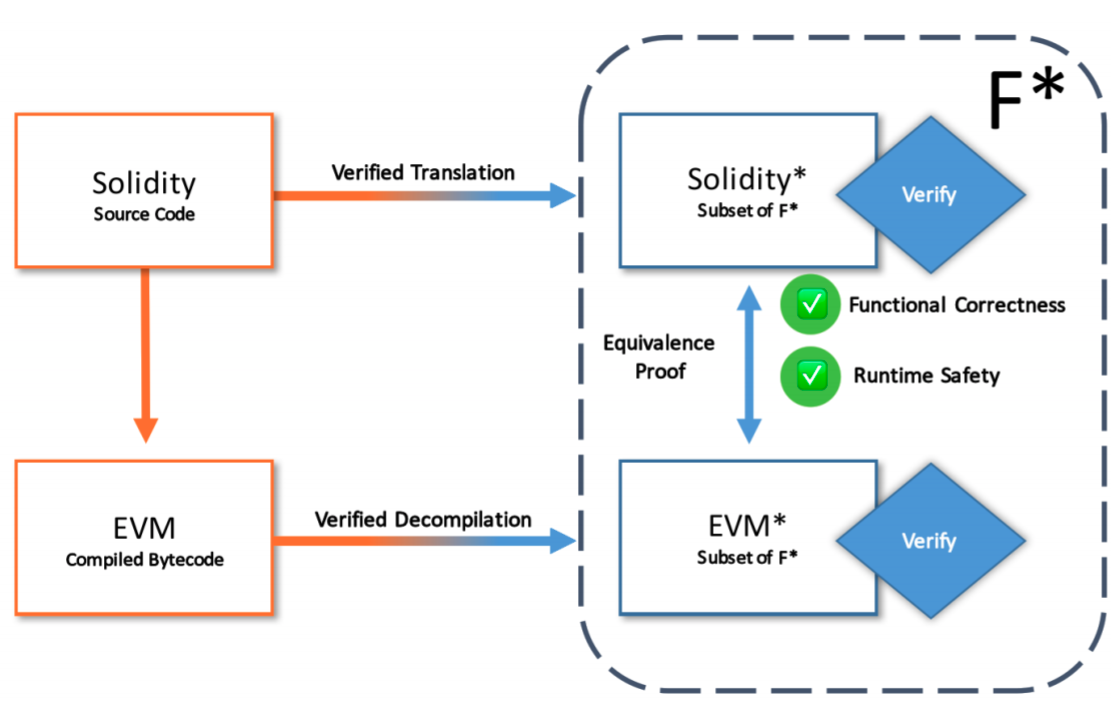
\includegraphics[scale=0.2]{Fstar}
\end{center}
\caption{\label{fig:oyente} The F* Tool's Structure}
\end{figure}


The most widely-known usage of this approach is through the use of the F*-Framework by Bhargavan. The authors aim to ensure the functional correctness and runtime safety of a given Solidity smart contract. The paper proposes an architecture of two translators, one taking in Solidity Code, and one taking in EVM Bytecode. Each of these translators translates their input into the functional language F*, on which runtime safety and functional correctness checks are performed. In the rare case (the authors claim this is the case for only 396 out of 112,802 contracts on Etherscan) where both the Solidity Code and EVM Bytecode for a given contract is available, the architecture can additionally be used to verify the functionality of the Solidity Compiler by checking the equivalence of the two generated F* programs. 
Further research has been conducted in using even more formal methods and thereby employing existing theorem checkers such as Isabelle to verify certain properties of EVM Bytecode. Though formal verification of security properties eliminates false positives, in practice its usability is lower than other approaches presented here, as the possibility for automating formal proofs is more limited, and even in cases where it is possible, the authors claimed it often resulted in long and repetitive proofs for even small amounts of EVM Bytecode.

\subsubsection{Linters}
An additional form of bug prevention and thereby software security insurance is the maintenance of a clean code style. Similar to many other programming languages, various linters such as Solcheck and Solint exist to enforce such standards for the Solidity programming language.

\subsubsection{Code Metrics}
Code Metrics play a significant role in the Quality Assurance process of many traditional software projects which target it is to minimize bugs and maximize code quality. These two goals go hand-in-hand with maximizing security, for which reason Péter Hegedűs developed SolMet. SolMet is a static analysis tool that aims to collect the same data on solidity code as tools traditionally used in QA do. Examples for this data collected by SolMet range from simple metrics such as LOC (Lines of Code) to more complex metrics values like the McCC (McCabe’s cyclomatic complexity).


\subsubsection{Lowering Gas Spend}
A further important issue that is highly specific to Ethereum is the detection of code that uses an unnecessarily high amount of gas. The reason why this is a security issue rather than a general inconvenience is due to the language design of solidity which does not throw an exception when instructions such as send fail due to insufficient gas. This can lead to unintended behavior of the smart contract if not handled adequately and can be exploited by a malicious actor to manipulate the smart contract in his favor. To address this issue, the GASPER tool was developed to identify gas costly patterns identified by the authors. Similar to previously discussed tools like OYENTE, GASPER also works on Ethereum bytecode and utilizes symbolic execution on the control flow graph to detect gas costly patterns.


\begin{figure}
\begin{center}
\includegraphics[scale=0.15]{Slither}
\end{center}
\caption{\label{fig:oyente} The Slither Tool's Structure}
\end{figure}

\subsubsection{State-of-the-art and Slither}
At the time of this writing, the state-of-the-art for static software security analysis is Slither. Slither works by taking in the abstract syntax tree provided by the Solidity compiler rather than the EVM bytecode in order to preserve more information regarding the structure of the previous solidity code. Based on this information, Slither converts the input to its internal representation, SlithIR, which uses static single assignment to ease the next step. In the third step, Slither performs some general analyses using which can serve as a base for detecting various vulnerabilities (which can be extended by the user) in the final stage. The authors claim it to be significantly faster and more accurate than competing analyzers.

\subsection{Dynamic Analysis Methods}

We define dynamic analysis as analysis performed on smart contracts in a runtime environment with the execution of the given smart contract.


Through dynamic analysis is more complex due to reasons previously explained for smart contracts, significant progress has been made in the field. In fact, state-of-the-art security audits of smart contracts very rarely solely perform static or dynamic analysis. Most use a combination of methods from both fields, as their weaknesses cover each other: Static analysis methods are generally better at exploring a wider variety of control flow paths but have an inclination of leading to false positives. On the other hand, due to the challenge of simulating all possible on- and off-chain events for a given smart contract, dynamic analysis methods tend to have more difficulty exploring all possible control flow paths of a given smart contract, but rarely lead to false positives. However, a key flaw in most static analysis methods is that most tools currently only work for "flat" invocations of contracts, that is calls to smart contracts that occur one single time.


\subsubsection{Execution Traces and MAIAN}
The resolution to this issue was addressed by Nikolic et al. in their paper introducing the MAIAN security analyzer. They introduce the term of trace vulnerabilities which are smart contract vulnerabilities caused by a potentially infinite sequence of invocations of the contracts functions. Using this term, they introduce three new classes of unsafe contracts: Greedy contracts, prodigal contracts, and suicidal contracts. They classify greedy contracts as contracts that lock their funds and cannot be destroyed (as destroying a contract returns the entrusted funds to a given address). Prodigal contracts are defined as contracts that give away funds to addresses that are not owners, previous interactors with the contract, or have any other direct relation to the contract. Finally, the paper describes suicidal contracts as contracts that allow an arbitrary/unintended address to command it to execute the SUICIDE instruction. All three of these classifications are based on errors behind previous large-scale Ethereum attacks. 

\begin{figure}
\begin{center}
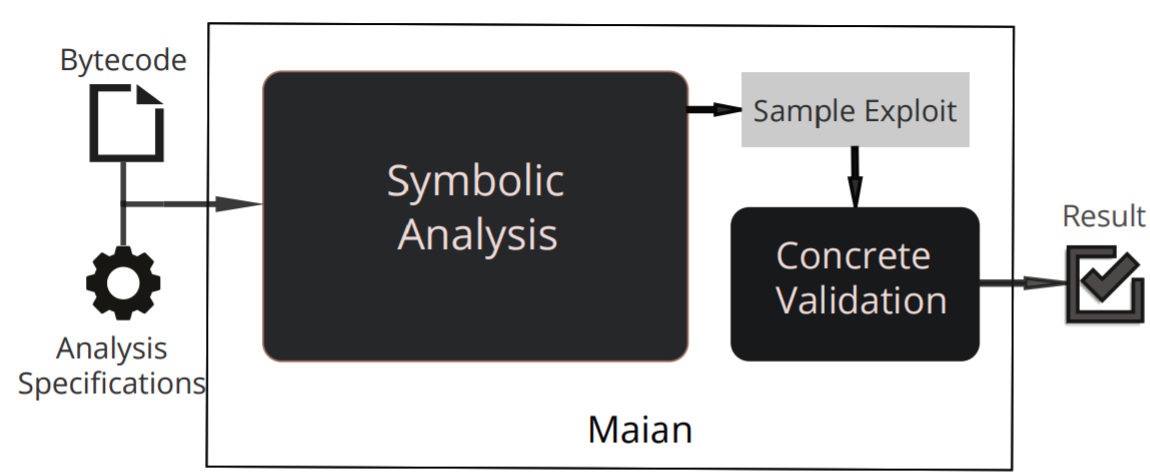
\includegraphics[scale=0.2]{MAIAN}
\end{center}
\caption{\label{fig:oyente} The MAIAN Tool's Structure}
\end{figure}

The tool introduced, MAIAN, leverages a combination of static and dynamic analysis methods as described in the introduction: It takes the Ethereum Bytecode along with analysis specifications as inputs. The analysis specification provides information about the type of vulnerabilities to search for along with other parameters to control MAIAN. It then first performs symbolic analysis on the given bytecode, using the previously introduced OYENTE as a basic framework. Once it detects a problematic set of inputs, it saves these and attempts to validate the exploit on a private fork of the Ethereum Network before returning it to the user to lower the number of false positives. Additionally, this execution of the potential exploit on a private fork ensures the maintenance of the state of the public Ethereum Network.


\subsubsection{Graph Construction}
In a paper by Chen, dynamic analysis of multiple smart contracts on the public Ethereum blockchain was conducted by creating three types of graphs, a Money Flow Graph, a Contract Creation Graph, and a Contract Invocation Graph. Using these three graphs, the authors were able to combat three security threats: 

\noindent First, given a malicious contract, the paper describes an algorithm using the Contract Creation Graph and Contract Invocation Graph to systematically detect all contracts and accounts under the control of the attacker. This methodology is useful in order to ensure that the contracts and addresses one's smart contract will interact with are not under the control of a bad actor.

\noindent Second, using the Contract Creation Graph once more, the authors provide an approach to detecting abnormal contract creation patterns, which is can be an indicator for a DoS (Denial of Service) Attack or a plot to steal tokens from a different smart contract. As previously stated, information that can be useful to have prior to deploying one's contract.

\noindent Finally, the authors also propose that the constructed graphs can be utilized for deanonymization techniques, however, this is more relevant to general Ethereum security rather than individual smart contracts.

\subsubsection{Testing}
The likely most prevalent strategy to prevent having security vulnerabilities in one's code is to write unit tests. These, however, can never detect every possible flaw, and, in the case of smart contracts generating every dangerous state manually is exceedingly difficult. For this reason, research has gone into both mutation testing and fuzzing. \linebreak



{\noindent \bf Mutation Testing}

\noindent For the case of Mutation Testing, the most significant paper is by Honig, where the authors introduce the Vertigo framework for mutation testing which runs on Truffle, a simulated Ethereum environment. This works by introducing the Solidity source code along with a working test suite to the framework. The framework then generates mutants (clones of the original contract with slight alterations in the source code) on which the test suite is run again, returning how many and which mutants passed the test suite.


\begin{figure}
\begin{center}
\includegraphics[scale=0.16]{echidna}
\end{center}
\caption{\label{fig:echidna} The Echidna Tool's Structure}
\end{figure}



{\noindent \bf Fuzzing}


\noindent The most widespread automated fuzzing tool is called Echidna and is based on Grieco's 2020 paper and also supports Truffle as a testing environment. Echidna takes in the smart contract source code along with a set of properties to verify and builds directly on top of the previously discussed Slither in order to gain easy access to the contracts ABI and other potentially useful constants and functions. Then, similar to Haskell's QuickCheck, Echidna continuously generates random transactions conforming to the contracts ABI. If one or a combination of these violates one of the preset properties,  Echidna minimizes said example and outputs it to the user.

\subsection{Other}
Along with static and dynamic analysis approaches, the Ethereum ecosystem provides some other resources to aid in making smart contracts more secure: One of these is the Smart Contract Weakness Classification Registry based on EIP-1470, where one can find various examples and counterexamples to common smart contract security flaws. Another is the introduction of higher-level languages such as Obsidian or Vyper - These may not give one quite the same level of control over the EVM as Solidity does, however the greater abstraction also helps alleviate some of the flaws of Solidity like its long array of best practices concerning deprecated and dangerous operations that beginners may accidentally use.

%-------------------------------------------------------------------------------
\section{Summary}
%-------------------------------------------------------------------------------

%-------------------------------------------------------------------------------
\section{References}
%-------------------------------------------------------------------------------
https://www4.comp.polyu.edu.hk/~csxluo/Gasper.pdf
\linebreak
\linebreak
https://www.mdpi.com/2227-7080/7/1/6/htm
\linebreak
\linebreak
https://loiluu.com/papers/oyente.pdf
\linebreak
\linebreak
https://drops.dagstuhl.de/opus/volltexte/2020/13015/pdf/OASIcs-SLATE-2020-2.pdf
\linebreak
\linebreak
\verb|http://pages.cpsc.ucalgary.ca/~joel.reardon/blockchain/readings/ndss2018_09-1_Kalra_paper.pdf|
\linebreak
\linebreak
https://arxiv.org/pdf/1806.01143.pdf
\linebreak
\linebreak
https://github.com/federicobond/solcheck
\linebreak
\linebreak
https://github.com/SilentCicero/solint
\linebreak
\linebreak
https://www.mdpi.com/2227-7080/7/1/6/htm
\linebreak
\linebreak
https://hal.inria.fr/hal-01400469/document
\linebreak
\linebreak
\verb|https://ts.data61.csiro.au/publications/csiro_full_text/Amani_BBS_18.pdf|
\linebreak
\linebreak
https://dl.acm.org/doi/pdf/10.1145/3381036
\linebreak
\linebreak
https://link.springer.com/content/pdf/10.1007%2F978-3-030-31500-9_19.pdf
\linebreak
\linebreak
https://arxiv.org/pdf/1908.09878.pdf
\linebreak
\linebreak
https://arxiv.org/pdf/1807.03932.pdf
\linebreak


%-------------------------------------------------------------------------------
\bibliographystyle{plain}
\bibliography{\jobname}

%%%%%%%%%%%%%%%%%%%%%%%%%%%%%%%%%%%%%%%%%%%%%%%%%%%%%%%%%%%%%%%%%%%%%%%%%%%%%%%%
\end{document}
%%%%%%%%%%%%%%%%%%%%%%%%%%%%%%%%%%%%%%%%%%%%%%%%%%%%%%%%%%%%%%%%%%%%%%%%%%%%%%%%

%%  LocalWords:  endnotes includegraphics fread ptr nobj noindent
%%  LocalWords:  pdflatex acks